%\documentclass[amsmath,table,sans,amsfonts, handout]{beamer}
\documentclass[amsmath,table,sans,amsfonts]{beamer}
\usepackage[T1]{fontenc}
%%\usepackage{beamerthemeshadow}
%%\usepackage[headheight=1pt,footheight=10pt]{beamerthemeboxes}
%%\addfootboxtemplate{\color{structure!80}}{\color{white}\tiny \hfill Karl Svozil (TU Vienna)\hfill}
%%\addfootboxtemplate{\color{structure!65}}{\color{white}\tiny \hfill mur.sat \hfill}
%%\addfootboxtemplate{\color{structure!50}}{\color{white}\tiny \hfill Graz, 2010-12-11\hfill}
%\usepackage[dark]{beamerthemesidebar}
%\usepackage[headheight=24pt,footheight=12pt]{beamerthemesplit}
%\usepackage{beamerthemesplit}
%\usepackage[bar]{beamerthemetree}
\usepackage{graphicx}
\usepackage{pgf}
%\usepackage{eepic}
%\usepackage[usenames]{color}
%\newcommand{\Red}{\color{Red}}  %(VERY-Approx.PANTONE-RED)
%\newcommand{\Green}{\color{Green}}  %(VERY-Approx.PANTONE-GREEN)


%\RequirePackage[german]{babel}
%\selectlanguage{german}
%\RequirePackage[isolatin]{inputenc}

%\pgfdeclareimage[height=0.5cm]{logo}{tu-logo}
%\logo{\pgfuseimage{logo}}
\beamertemplatetriangleitem
%\beamertemplateballitem

\beamerboxesdeclarecolorscheme{alert}{red}{red!15!averagebackgroundcolor}
%\begin{beamerboxesrounded}[scheme=alert,shadow=true]{}
%\end{beamerboxesrounded}

%\beamersetaveragebackground{yellow!10}

%\beamertemplatecircleminiframe

\newtheorem{question}{Question}
\newtheorem{conjecture}[question]{Principle}
\newtheorem{challenge}[question]{Challenge}
\usepackage{tikz}
\newcommand{\bra}[1]{\left< #1 \right|}
\newcommand{\ket}[1]{\left| #1 \right>}

\newcommand{\iprod}[2]{\langle #1 | #2 \rangle}
\newcommand{\mprod}[3]{\langle #1 | #2 | #3 \rangle}
\newcommand{\oprod}[2]{| #1 \rangle\langle #2 |}

\newcommand{\proj}[3]{\begin{smallmatrix} #1 & #2 & #3 \end{smallmatrix}}
\newcommand{\projbf}[3]{\begin{smallmatrix} \mathbf{#1} & \mathbf{#2} & \mathbf{#3} \end{smallmatrix}}

\sloppy
\parskip .7em %vskip between paragraphs

\newcommand{\seq}[1]{\mathbf{#1}}
\newcommand{\floor}[1]{\left\lfloor #1 \right\rfloor}
\newcommand{\ceil}[1]{\left\lceil #1 \right\rceil}
\newcommand{\m}[1]{\widetilde{#1}}
\newcommand{\p}[1]{\scriptsize\textcolor{black}{$[#1]$}}

\begin{document}

\title{\bf \textcolor{blue}{Unscrambling the Quantum Omelette}}
\subtitle{\textcolor{purple!60}{\small http://tph.tuwien.ac.at/$\sim$svozil/publ/2013-Florence-pres.pdf
\\
http://arxiv.org/abs/1206.6024
}}
\author{Karl Svozil}
\institute{University of Technology Vienna, Austria\\
svozil@tuwien.ac.at
%{\tiny Disclaimer: Die hier vertretenen Meinungen des Autors verstehen sich als Diskussionsbeitr�ge und decken sich nicht notwendigerweise mit den Positionen der Technischen Universit�t Wien oder deren Vertreter.}
}
\date{Florence, June 17th, 2013}
\maketitle


% \frame{
% \frametitle{Contents}
% \tableofcontents
% }

\section{Roads to quantum confusions}

 \frame{
 \frametitle{Jaynes' Quantum Omelette}

{\color{purple}
{\em ``$\ldots$ our present QM formalism is not purely epistemological; it is a peculiar mixture describing
in part realities of Nature, in part incomplete human information about Nature --- all scrambled up
by Heisenberg and Bohr into an omelette that nobody has seen how to unscramble. Yet we think
that the unscrambling is a prerequisite for any further advance in basic physical theory. For, if we
cannot separate the subjective and objective aspects of the formalism, we cannot know what we
are talking about; it is just that simple. So we want to speculate on the proper tools to do this..''}
} \\
$\;$\\
Edwin Thompson Jaynes,
 {\em Probability in Quantum Theory} (1990)\\
 http://bayes.wustl.edu/etj/articles/prob.in.qm.pdf
}

 \frame{
 \frametitle{Ingredients to produce a quantum omelette}

\begin{itemize}
\pause
\item {\color{purple}{intrinsic}} self-perception:
no observer has a ``direct, detached, objective, extrinsic'' viewpoint;
all observers are ``embedded'' in the system they observe (``Cartesian prison'');
\pause
\item all observations are based on {\color{purple}{detector clicks}};
\pause
\item based on these clicks, and through ``{\color{purple}{projections and conventions}}''
of our mind we reconstruct what we consider the physical universe;
\end{itemize}
}

 \frame{
 \frametitle{Mind Projection Fallacy according to Jaynes}

{\color{purple}
{\em ``$\ldots$ we are all under an ego-driven temptation to project our private
thoughts out onto the real world, by supposing that the creations of one's own imagination are real
properties of Nature, or that one's own ignorance signifies some kind of indecision on the part of
Nature.''}
} \\
$\;$\\
Edwin Thompson Jaynes,
 {\em Clearing up Mysteries - The Original Goal} (1989)\\
 http://bayes.wustl.edu/etj/articles/cmystery.pdf\\
$\;$\\
{\color{blue}{I believe that this sort of ``over-interpretation of empirical data''
is at the heart of many misconceptions
about quantized systems. }}
}

 \frame{
 \frametitle{Quantum examples of the Mind Projection Fallacy}
\begin{itemize}
\pause
\item {\color{purple}{irreducible}} (and not merely ``FAPP''=for all practical purposes)
{\color{purple}{randomness}} {\color{blue}{-- formally, by reduction to recursion theoretic unknowables
(eg, the halting problem or the rule inference problem), randomness as well as determinism turns out to be
{\color{purple}{provably unprovable}}}};
\pause
\item ``experimental proofs'' of the {\color{purple}{Kochen-Specker theorem}}:
``how can you measure a [proof by] contradiction?'' (Rob Clifton, 1995);
\pause
\item physical existence of {\color{purple}{``counterfactuals;''}}
(Specker's ``Infuturabilien'' referring to scholastic debates): hypothetical observables
that you could have, but did not measure;
instead you measured some different, complementary, observable;
\end{itemize}
}
 \frame{
 \frametitle{Quantum examples of the Mind Projection Fallacy cntd.}
\begin{itemize}

\item ``experimental proofs'' of {\color{purple}{contextuality}}: what is really measured are
``violations of Boole-Bell type inequalities {\em via}
successive measurements of counterfactual, complementary observables that are not co-measurable;''
\pause
\item
assumption of a {\color{purple}space-time theater} in which events occur;
 rather than the ``operationalization'' of space-time {\em via} events.
\end{itemize}
}


\frame{

\centerline{\Large {\color{magenta} Part I: Single pure state conjecture}}

\begin{center}\color{orange}
$\widetilde{\qquad \qquad }$
$\widetilde{\qquad \qquad}$
$\widetilde{\qquad \qquad }$
\end{center}
 }

\section{Abbott-Calude-Conder-Svozil theorem}



 \frame{
 \frametitle{So, how might one be able to ``unscramble'' the Quantum Omelette?}

{\color{purple}{Try the Kochen-Specker theorem as a guiding principle.} }

The (strong) Kochen-Specker theorem is usually proven by taking a finite subset of interconnected
(the dimension of the vector space must be three or higher for interconnectivity)
contexts
($=$maximal observables$=$orthogonal bases$=$unitary operators),
and by demonstrating that no two-valued measure (interpretable as classical truth assignment)
exists on those structures of observables
if noncontextuality is required -- meaning that the measure is independent of the context.

{\color{gray}  Weaker forms allow two-valued measures, alas too few to be separating some observables; or to allow a
homeomorphic embedding into Boolean algebras.}
}

 \frame{
 \frametitle{Certified breakdown of value indefiniteness in ACCS theorem}

Consider a modified, and, in a particular sense,
``improved'' version of the Kochen-Specker theorem
which certifies ``breakdown of (noncontextual) value definiteness'' at a particular observable:

{\color{blue}{
Let $\ket{\textsf{\textbf{a}}},\ket{\textsf{\textbf{b}}}\in \mathbb{C}^3$ be unit vectors such that
$\sqrt{\frac{5}{14}} \le |\iprod{\textsf{\textbf{a}}}{\textsf{\textbf{b}}}| \le \frac{3}{\sqrt{14}}\raisebox{.8mm}{.}$
Then there exists a set of vectors (forming interlinked contexts or blocks)
$\Gamma ( \vert \textsf{\textbf{a}} \rangle , \vert \textsf{\textbf{b}} \rangle)$
containing $\ket{\textsf{\textbf{a}}}$ and $\ket{\textsf{\textbf{b}}}$,
such that there is no two-valued state (admissible assignment function) under which $\mathcal{O}$ is non-contextual,
$v (\ket{\textsf{\textbf{a}}}\bra{\textsf{\textbf{a}}}) $ has the value 1 and $\ket{\textsf{\textbf{b}}}\bra{\textsf{\textbf{b}}}$ is value definite.
}}

Abbott, Calude, Conder \& K.S. (ACCS), DOI: 10.1103/PhysRevA.86.062109, eprint arXiv:1207.2029
}


 \frame{
 \frametitle{Pitowsky's Logical Indeterminacy Principle}

{\color{blue}{
Let $\vert \textsf{\textbf{a}} \rangle$ and $\vert \textsf{\textbf{b}} \rangle$
be two non-orthogonal rays in a Hilbert space  of
finite dimension greater than two.
Then there is a finite set of rays $\Gamma ( \vert \textsf{\textbf{a}} \rangle , \vert \textsf{\textbf{b}} \rangle)$
such that
$\vert \textsf{\textbf{a}} \rangle , \vert \textsf{\textbf{b}} \rangle \in
\Gamma (\vert \textsf{\textbf{a}} \rangle , \vert \textsf{\textbf{b}} \rangle)$
such that any two-valued state $v$ on $\Gamma ( \vert \textsf{\textbf{a}} \rangle , \vert \textsf{\textbf{b}} \rangle)$
must satisfy $v(\vert \textsf{\textbf{a}} \rangle)= v( \vert \textsf{\textbf{b}} \rangle )=0$.
}}

Pitowsky ``Infinite and Finite Gleason's Theorems and the Logic of Indeterminacy'', Journal of Mathematical Physics 39, 218-228 (1998);
as well as Hrushovski \& Pitowsky "Generalizations of Kochen and Specker's Theorem and the Effectiveness of Gleason's Theorem'', Studies in the History and Philosophy of Modern Physics 35, 177-194 (2004)

}

 \frame{
 \frametitle{Value definiteness restricted to star-shaped configurations}

{\color{blue}{
Hence, given a two valued measure $v$ in a Hilbert space  of
finite dimension greater than two,
and some ray $\vert \textsf{\textbf{c}} \rangle$ with $v(\vert \textsf{\textbf{c}} \rangle)=1$.
Relative to the Kochen-Specker assumptions,
the only consistent, value definite truth assignments is
``inside $\vert \textsf{\textbf{c}} \rangle$'s star.''
``Outside of $\vert \textsf{\textbf{c}} \rangle$'s star''
all ``observables'' are value indefinite.
(This is true relative to the Kochen-Specker assumptions, including non-contextuality.)
}}

\begin{center}
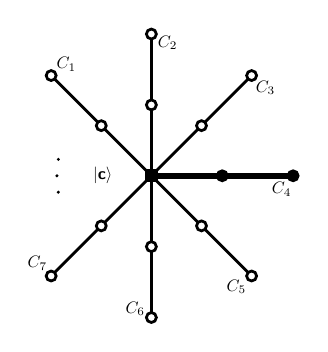
\begin{tikzpicture}    [scale=0.6, transform shape]
\tikzstyle{every path}=[line width=1pt]
\tikzstyle{every node}=[draw,line width=1pt,inner sep=0]

\tikzstyle{c1}=[rectangle,minimum size=6]

\tikzstyle{d1}=[circle,draw=none,fill,minimum size=2]

\tikzstyle{l7}=[draw=none,circle,minimum size=45]

\draw[black] (0:0) -- (135:3)
	coordinate[c1,at start] (0)
	coordinate[c1,circle,midway,fill=white] (1)
	coordinate[c1,circle,at end,fill=white,label=35:$C_1$] (2);

\draw[black] (0.center) -- (90:3)
	coordinate[c1,at start] (0)
	coordinate[c1,circle,midway,fill=white] (3)
	coordinate[c1,circle,at end,fill=white,label=350:$C_2$] (4);

\draw[black] (0.center) -- (45:3)
	coordinate[c1,at start] (0)
	coordinate[c1,circle,midway,fill=white] (5)
	coordinate[c1,circle,at end,fill=white,label=305:$C_3$] (6);

\draw[black] (0.center) -- (315:3)
	coordinate[c1,at start] (0)
	coordinate[c1,circle,midway,fill=white] (9)
	coordinate[c1,circle,at end,fill=white,label=215:$C_5$] (10);

\draw[black] (0.center) -- (270:3)
	coordinate[c1,at start] (0)
	coordinate[c1,circle,midway,fill=white] (11)
	coordinate[c1,circle,at end,fill=white,label=170:$C_6$] (12);

\draw[black] (0.center) -- (225:3)
	coordinate[c1,at start] (0)
	coordinate[c1,circle,midway,fill=white] (13)
	coordinate[c1,circle,at end,fill=white,label=125:$C_7$] (14);

\draw[black,line width=2pt] (0.center) -- (0:3)
	coordinate[c1,fill,at start] (0)
	coordinate[c1,circle,fill,midway] (7)
	coordinate[c1,circle,fill,at end,label=260:$C_4$] (8);

\coordinate[l7,label=180:$\vert \textsf{\textbf{c}} \rangle$] (0) at (0.center);

\coordinate[d1,black] (.) at (190:2);
\coordinate[d1,black] (.) at (180:2);
\coordinate[d1,black] (.) at (170:2);
\end{tikzpicture}
\end{center}

}


\section{Ontological single pure state conjecture}

\frame{
\frametitle{How can one utilize the Kochen-Specker and related theorems?}
\begin{itemize}
\pause
\item {\color{purple}{quantum random number generator}} ``certified by quantum value indefiniteness:''
prepare  state $\vert \textsf{\textbf{c}} \rangle$, measure projector $\ket{\textsf{\textbf{b}}}\bra{\textsf{\textbf{b}}}$ (please see ACCS paper for experimental setup for quantum coin tosses);
\pause
\item
While the ACCS theorem certifies only one observable to be value indefinite (given noncontextuality),
and while as already pointed out in the ACCS paper,
extensions will never be able to go beyond value indefiniteness
of all but a ``star shaped'' configuration of contexts discussed later -- the
{\color{purple}{ontological single pure state conjecture}}
{\color{teal} suggests to ``throw the baby out with the bathwater'' by denying the physical co-existence of
all but one measuement context prior to measurement:
At any given time the system is in a single definite context.
In terms of observables, this translates into
``ontologically there does not exist any observable beyond the observables representing a single definite context.''
}
\end{itemize}
}

\frame{
\frametitle{Ontological single pure state conjecture cntd. }
\begin{itemize}
\item
The ontological single pure state conjecture
claims that a single quantum state is a {\color{purple}{complete}}
theoretical representation of a physical system.
\pause
\item
Thereby the ontological single pure state conjecture {\color{purple}{ abandons omniscience:}}
it states that all other (even hypothetically ``value definite'' yet counterfactual) observables
different from the observables associated with the unique state,
and possibly
ascribed to such a system, are not value definite at all.
\end{itemize}
}
\frame{
\frametitle{Ontological single pure state conjecture cntd.}
\begin{itemize}
\item
Make no mistake: such value indefinite observables may
seem to be ``measurable'' in the sense that their
``measurement'' yields outcomes; that is, detector clicks.
But these {\color{purple}outcomes cannot reflect any value definite property of the object prior to measurement}
because, according to the single pure state conjecture,
such a value definite property  simply does not exist.
Rather the detector clicks associated with the ``measurement'' might result
from  properties that also depends
{\em ``on the complete disposition  of the apparatus''}, as well as on the object, combined.
\pause
\item
In contradistinction, orthodox quantum mechanics
treats {\color{purple}all} these observables on an {\color{purple}equal footing.}
\end{itemize}
}

\section{What constitutes a pure quantum state?}
\frame{
\frametitle{What is the formal characterization of a pure quantum state?}


Informally,
A pure state is characterized by
the {\color{purple} maximal information} encodable into a physical system.



Formally, a pure state can be represented by
\begin{itemize}
\item
 a two-valued $\{0,1\}$-measure on an {\color{purple} orthonormal basis};
\item
a {\color{purple}  maximal operator}  from which all commuting operators can be functionally derived;
\item
 a two-valued $\{0,1\}$-measure on a {\color{purple}  context, subalgebra} or {\color{purple} block};
\item
 a {\color{purple} unitary transformation} associated with some orthonormal basis, and the choice of an element of that basis.
\end{itemize}

}



\frame{
\frametitle{Phantom contexts and context translation}

{\color{purple}Phantom context:}
{\color{teal}
Any context that is not the single context/state (in which the system is prepared).   }


{\color{purple}Context translation principle:}
{\color{teal}
A  mismatch between the preparation and the measurement may result in the ``translation''
of the original information encoded by a quantum system into the answer requested,
whereby noise is introduced by the many degrees of freedom of a suitable ``quasi-classical'' measurement apparatus.   }


}


\frame{
\frametitle{Ontology of star shaped Greechie diagram of ``phantom'' contexts}

\begin{center}
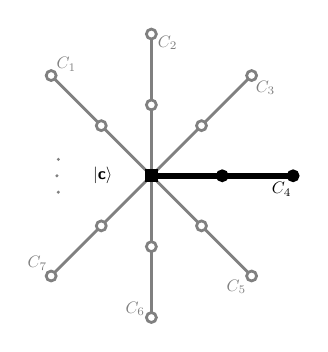
\begin{tikzpicture}    [scale=0.6, transform shape]
\tikzstyle{every path}=[line width=1pt]
\tikzstyle{every node}=[draw,line width=1pt,inner sep=0]

\tikzstyle{c1}=[rectangle,minimum size=6]

\tikzstyle{d1}=[circle,draw=none,fill,minimum size=2]

\tikzstyle{l7}=[draw=none,circle,minimum size=45]

\draw[gray] (0:0) -- (135:3)
	coordinate[c1,at start] (0)
	coordinate[c1,circle,midway,fill=white] (1)
	coordinate[c1,circle,at end,fill=white,label=35:$C_1$] (2);

\draw[gray] (0.center) -- (90:3)
	coordinate[c1,at start] (0)
	coordinate[c1,circle,midway,fill=white] (3)
	coordinate[c1,circle,at end,fill=white,label=350:$C_2$] (4);

\draw[gray] (0.center) -- (45:3)
	coordinate[c1,at start] (0)
	coordinate[c1,circle,midway,fill=white] (5)
	coordinate[c1,circle,at end,fill=white,label=305:$C_3$] (6);

\draw[gray] (0.center) -- (315:3)
	coordinate[c1,at start] (0)
	coordinate[c1,circle,midway,fill=white] (9)
	coordinate[c1,circle,at end,fill=white,label=215:$C_5$] (10);

\draw[gray] (0.center) -- (270:3)
	coordinate[c1,at start] (0)
	coordinate[c1,circle,midway,fill=white] (11)
	coordinate[c1,circle,at end,fill=white,label=170:$C_6$] (12);

\draw[gray] (0.center) -- (225:3)
	coordinate[c1,at start] (0)
	coordinate[c1,circle,midway,fill=white] (13)
	coordinate[c1,circle,at end,fill=white,label=125:$C_7$] (14);

\draw[black,line width=2pt] (0.center) -- (0:3)
	coordinate[c1,fill,at start] (0)
	coordinate[c1,circle,fill,midway] (7)
	coordinate[c1,circle,fill,at end,label=260:$C_4$] (8);

\coordinate[l7,label=180:$\ket{\textsf{\textbf{c}}}$] (0) at (0.center);

\coordinate[d1,gray] (.) at (190:2);
\coordinate[d1,gray] (.) at (180:2);
\coordinate[d1,gray] (.) at (170:2);
\end{tikzpicture}
\end{center}

Greechie orthogonality diagram of a star-shaped configuration,
representing a common basis element/projector $\ket{\textsf{\textbf{c}}}$ with an overlaid two-valued assignment reflecting $v({\textsf a})=1$.
Compare also the difference and similarities to Abbott, Calude, Conder \& K.S., DOI: 10.1103/PhysRevA.86.062109, eprint arXiv:1207.2029

}

\frame{
\frametitle{Specker's ``bug'' diagram of ``phantom'' contexts}


\begin{center}
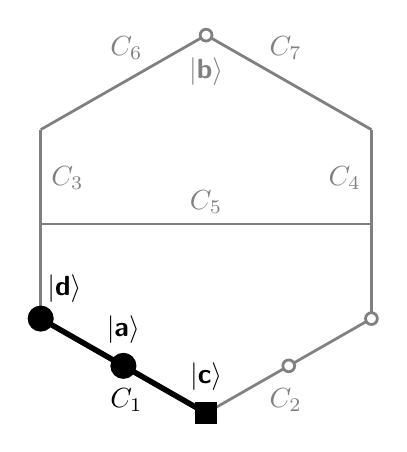
\begin{tikzpicture} [scale=0.3]

\tikzstyle{every path}=[line width=1pt]
\tikzstyle{c1}=[rectangle,minimum size=8]

%\draw[help lines,orange] (-7,-8) grid (7,8);


\draw[gray]  (7,4) -- (7,-4);
\node [above left, gray] at (7,1) {$C_4$};

\draw[gray]  (7,-4) -- (0,-8) ;
\node [below left, gray] at (4.5,-6.5) {$C_2$};
\draw[gray,fill=white] (7,-4) circle [radius=0.25];
\draw[gray,fill=white] (3.5,-6) circle [radius=0.25];

\draw[gray]  (-7,-4) -- (-7,4);
\node [above right, gray] at (-7,1) {$C_3$};

\draw[gray]  (-7,4) -- (0,8) ;
\node [above right, gray] at (-4.5,6.5) {$C_6$};

\draw[gray]  (0,8) -- (7,4);
\draw[gray,fill=white] (0,8) circle [radius=0.25];
%\node [green, label=below:$\vert \textsf{\textbf{b}} \rangle $] at (0,8) {};
\node [below, gray] at (0,7.5) {$\vert \textsf{\textbf{b}} \rangle $};
\node [above left, gray] at (4.5,6.5) {$C_7$};


\draw[gray]  (-7,0) -- (7,0);
\node [above, gray] at (0,0) {$C_5$};

\draw [line width=2pt,black]  (0,-8) -- (-7,-4)
        coordinate[c1,circle, at end,fill=black] (0)
        coordinate[c1,circle,midway,fill=black] (1)
        coordinate[c1,rectangle,at start,fill=black] (2);
\node [below right, black] at (-4.5,-6.5) {$C_1$};
%\node [label=above:$\vert \textsf{\textbf{a}} \rangle $, black] at (0,-8) {};
\node [above, black] at (0,-7.5) {$\vert \textsf{\textbf{c}} \rangle $};
\node [above, black] at (-3.5,-5.5) {$\vert \textsf{\textbf{a}} \rangle $};
\node [above, black] at (-6,-3.75) {$\vert \textsf{\textbf{d}} \rangle $};

\end{tikzpicture}
\end{center}

``Bug-type''  Greechie orthogonality diagram
with an overlaid two-valued assignment reflecting ``$v(\ket{\textsf{\textbf{c}}})=1$ implies $v(\ket{\textsf{\textbf{b}}})=0$.''
This configuration is part of the original
proof of the Kochen-Specker theorem.
It is assumed that the system is prepared in state $C_1$, depicted by a block colored in thick filled black;
all the other contexts $C_2$--$C_7$ are   ``phantom contexts'' colored in gray.

}




\frame{

\centerline{\Large {\color{magenta} Part II: Persistent Issues}}

\begin{center}\color{orange}
$\widetilde{\qquad \qquad }$
$\widetilde{\qquad \qquad}$
$\widetilde{\qquad \qquad }$
\end{center}
 }




\section{Persistent issues}

\subsection{Do measurements exist?}

\frame{
\frametitle{Everett and Wigner's observation of a subjective observer-object cut}

Around the same time (in the late 50's),
Everett  and  Wigner
observed that,
if a unitary (bijective, one-to-one, reversible, Laplacian-type deterministic) quantum evolution were universally valid,
then any distinction or cut between the observer and the measurement apparatus necessarily remains not absolute or ontic,
but epistemic, subjective and conventional.

Because, suppose that one has defined a cut or difference between an observed quantum and a ``quasi-classical'' measurement device,
one could, at least in principle and if the unitary quantum evolution is universally valid,
``draw a larger perimeter.'' This ``enlargement'' could contain the entire previous combination,
{\em including} the quantum, the cut, and the measurement device.
If the quantum laws are universally valid, such a quantized system should also undergo
a unitary quantum evolution.
Hence, any ``irreversibility'' decays into ``thin air.''
}

\frame{
\frametitle{There is no `emergence' of many-to-one from one-to-one functions; and thus no strictly
``irreversible measurement.''}


{\color{purple}{If quantum mechanics is universally valid,
and if it is governed by unitary, reversible, one-to-one evolution,
how does irreversibility arise from reversibility?}   }

Suppose (wrongly) a hypothetical many-to-one function $h(x)=h(y)$ for $x\neq y$ exists which would somehow
`emerge' from injective functions.
Any such function would have to originate from the domain of one-to-one functions such that,
for all functions $f$ of this class,  $x\neq y$ implies  $f(x)\neq f(y)$
-- or, equivalently, the contrapositive statement (provable by comparison of truth tables)
$f(x) = f(y)$ implies $x = y$,  a clear contradiction with the assumption.


Indeed, by {\color{purple}Caylay's theorem}
the {\em unitary transformations} on some Hilbert space ${\mathfrak H}$
form a particular permutation group (consisting of those permutations preserving the inner product),
which is a subgroup of the {\em symmetric group}
of all permutations on ${\mathfrak H}$.

}


\subsection{Quantum jellification}

\frame{
\frametitle{Quantum jellification}

Alas, without measurement, Schr\"odinger (in his Dublin seminars 1952) pointed out that
quantum theorists should be troubled that, due to the coherent superposition
resulting from the co-existence of classically mutually exclusive alternatives,
their  {\color{blue} ``surroundings rapidly turning into a quagmire, a sort of a featureless jelly or plasma,
all contours becoming blurred, we ourselves probably becoming jelly fish.''}


{\color{teal}  The single pure state conjecture and
the context translation principle
would resolve this conundrum by maintaining that there is only one state ``perceived'' from many
epistemic perspectives; some of them causing noise which FAPP appears irreducible random to intrinsic observers.   }
}






\subsection{Analogues in classical statistical mechanics}
\frame{
\frametitle{Analogues in classical statistical mechanics}

Just as Newtonian physics and electromagnetism appear to be reversible,
the quantum measurement conundrum is characterized by the reversibility of
the unitary quantum evolution.

In this respect, the (ir-)reversibility of quantum measurements
bears some analogy to {\color{purple}Loschmidt's reversibility paradox}
--
that, for large isolated systems with reversible laws of motion, one should never
observe irreversibility, and thus a decrease in entropy
--
and {\color{purple}Zermelo's recurrence objection}
--
that, as an isolated system will infinitely often approach its initial
state, its entropy will infinitely often approach the initial entropy and thus cannot constantly
increase
--
in classical statistical mechanics.


And just as in statistical mechanics, irreversibility appears {\color{purple}means-relative} and
{\color{purple}FAPP correct}, yet cannot strictly be true.

}




\subsection{The epistemic or ontic (non-)existence of mixed states}
\frame{
\frametitle{Btw, is it in principle possible to produce a mixed state from a pure one?}

Again, from a purely formal point of view,
it is impossible to obtain a mixed state from a pure one.
Because again, any unitary operation amounts to a mere basis transformation or permutation,
and this cannot give rise to any increase in stochasticity or ``ignorance.''
Since the generation of ``ontologically mixed states'' from pure ones would require a many-to-one functional mapping,
we conclude that, just as irreversible measurements, genuine ``ontological mixed states'' originating from pure states cannot exist.
Therefore, any ontological mixed state has to be either carried through from previously existing mixed states; if they exist.

{\color{violet}
If you dont believe me, then I suggest you come
up with a concrete experiment that would ``produce'' a mixed state from a pure one.
}

}



\subsection{Some further speculations regarding quantum random number generators}
\frame{
\frametitle{Some further speculations regarding  quantum random number generators}

It is often believed (Born's ``1926 inclinations''), that quantum randomness
miraculously emerges in a {\color{purple} \it creatio ex nihilo}
from devices which perform in the Laplacian deterministic-unitary regime,
such as beam splitters.
But how can this happen from unitary transformations alone?

{\color{purple} Where does the quantum randomness reside?}

I suggest to circumvent this conundrum is by postulating that
(i) at every instant, only a single state (or context) exists;
and that
(ii)
through {\em context translation,}
in which a mismatch between the preparation and the measurement results in the ``translation''
of the original information encoded by a quantum system into the answer requested.
Thereby
noise is introduced by the many degrees of freedom of a suitable ``quasi-classical'' measurement apparatus.
}


\frame{

\centerline{\Large {\color{magenta} Part III: Some thoughts on music \& arts in general}}

\begin{center}\color{orange}
$\widetilde{\qquad \qquad }$
$\widetilde{\qquad \qquad}$
$\widetilde{\qquad \qquad }$
\end{center}
 }


\section{What is art?}
\frame{
\frametitle{What is art?}

\begin{itemize}
\item
{\color{purple} ``Art is all there is''} -- maybe too general;
\item
{\color{purple} ``Art comprises those methods and practices that explore the humain realm''} --
 maybe still too general,                            because
this implies that art includes {\color{purple} science} and {\color{purple} pain \& torture}, as well as {\color{purple} philosophy};
\item
{\color{purple}  ``Art explores beauty''}  -- to narrow for some who, for instance, promote provocations \& ``actionism'';
\end{itemize}

So, my suspicion is that {\color{purple} there is no generally accepted definition of what constitutes ``Art.''}
}

\frame{
\frametitle{Suppose we restrict ourselves to beauty}

\begin{itemize}
\item
{\color{purple} ``Art competes with strong desires and natural beauty:''} Even Botticelli's  {\it Primavera}
cannot compete with a beautiful woman, at least by measure of impression on the common man --
so, is art a {\color{purple}simulacrum}?
\item
Three principles of {\color{purple} Aesthetic Complexity:}

\begin{itemize}
\item
According to the first law of aesthetic complexity,
too condensed encoding makes a decryption of a work of art impossible and is perceived as chaotic by the untrained mind,
whereas too regular structures are perceived as monotonous, too orderly and not very stimulating.
Thus a necessary condition for an artistic form or design to appear appealing is its complexity to lie within a bracket between monotony and chaos.
\item
According to the second law of aesthetic complexity, due to human predisposition,
this bracket is invariably based on natural forms; with rather limited plasticity.
\item
The third law of aesthetic complexity states that aesthetic complexity trends
are dominated by the available resources, and thus also by cost and scarcity.
\end{itemize}


\end{itemize}

}

\frame{

\centerline{Sch\"onberg versus Cage, in {\em Cage, An Autobiographical Statement, 1989}   }

{\color{blue}
{
After two years it became clear
	to both of us [[Sch\"onberg and Cage]] that I [[Cage]] had no feeling
	for harmony. For Schoenberg, harmony was not just coloristic: it
	was structural. It was the means one used to distinguish one part
	of a composition from another. Therefore he said I'd never be able
	to write music. ``Why not?'' ``You'll come to a wall and won't be
	able to get through.'' ``Then I'll spend my life knocking my head
	against that wall.''}
}

{\color{magenta}In my opinion, contemporary modern art is characterized by this ``knocking our heads
	against various walls.'' }


{\color{magenta}Maybe contemporary art (\& life) needs to be more committed to beauty \& love. }
}

\frame{

\centerline{\Large {\color{magenta} Thank you for your attention!}}

\begin{center}\color{orange}
$\widetilde{\qquad \qquad }$
$\widetilde{\qquad \qquad}$
$\widetilde{\qquad \qquad }$
\end{center}
 }
 \end{document}
